\zotelo{../thesis.bib}

\chapter{Introduction}
\label{chap:intro}

Astrophysics builds upon observations of astronomical objects at various
radiation bands. Some of the most interesting objects in the sky are sources of
high energy radiation, including but not limited to pulsars, supernovae,
magnetars, super-massive black holes, etc. The high-energy spectra of these
objects up to hard X-ray and gamma-rays are often highly non-thermal, suggesting
that it is from high-energy particles. The study of particle acceleration and
conversion of other forms of energy into particle kinetic energy is therefore
vital in the study of high-energy astrophysics.

In many of the sources, the most notable source of energy for nonthermal
particles is the magnetic energy. For example in pulsars, magnetic field plays
an intermediary role, acting as a channel that converts the rotational energy of
the pulsar into the particle energy, which then is radiated away eventually and
produce the observed radio/X-ray/gamma ray emission from the pulsar or in the
surrounding pulsar wind nebula. In other sources such as magnetars it is the
magnetic energy itself that is directly converted to particle energy that is
radiated.

% TODO: Go into more details, and mention past work
Dissipation of magnetic energy and acceleration of particles is inherently a
highly nonlinear process, and a direct calculation is very difficult. The recent
development in computational power has enabled direct simulations of various
physical scenarios that can lead to particle acceleration, such as collisionless
shocks and magnetic reconnection, allowing rapid development in these fields.
Simulations have become a vital tool in understanding high energy plasma
astrophysics. With the advent of new architectures like the Graphics Processing
Unit (GPU), larger scale simulations are becoming more accessible, enabling
direct simulations of global systems like the magnetospheres of neutron stars.
% In the past people have tried different methods. Some
% attempt to model the whole system by treating the plasma as fluid, and use
% magnetohydrodynamics or force-free approximation. Some isolate part of the
% system and study the detailed local evolution of eletromagnetic fields. It is
% only recently that computational power has increased to the level that we could
% attempt a first-principle direct simulation of the system of interest.

This dissertation will be focusing on the physics of isolated neutron stars. In
the following sections we will give a broad overview of the history and basic
physics of rotation-powered pulsars, and the exotic magnetars which have
extremely high magnetic field. Finally we will give an outline of this thesis.

\section{Pulsars}
\label{sec:intro-pulsars}

\subsection{Early Observations}

The first observational discovery of the rotation-powered pulsars (RPP) dates
back to late 1960s \citep{hewish_observation_1968}. In this paper a periodic
radio source was reported to be emitting regular pulsation at a frequency of
$81.5\,\mathrm{MHz}$, with a period of $1.337\,\mathrm{s}$ at extreme accuracy.
The pulse width of the object gives an upper bound on its physical size, which
should not exceed $4.8\times 10^3\,\mathrm{km}$. The extreme constancy of the
intrinsic period suggests that the source is a massive object, rather than some
astrophysical plasma configuration. It was therefore conjectured that this
pulsed radio emission was coming from a compact star: a white dwarf or a neutron
star; the extreme regular pulsation is a result of its rapid rotation
\citep{gold_rotating_1968}.

\begin{figure}[h]
  \centering
  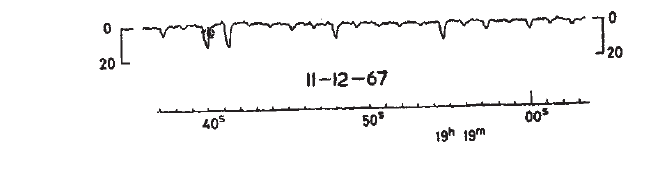
\includegraphics[width=0.6\textwidth]{pics/intro/pulses.png}
  \caption[A record of pulsating radio source]{A record of the pulsating radio
    source discovered in 1967 \citep{hewish_observation_1968}}
  \label{fig:pulse}
\end{figure}

More pulsars were soon discovered, e.g.\ the Vela with a period of
$89\,\mathrm{ms}$ \citep{large_pulsar_1968} and the Crab with a period of
$33\,\mathrm{ms}$ \citep{lovelace_pulsar_1968}. Slowing down of the periods were
also discovered in the known pulsars. The spin-down luminosity can be easily
estimated given the period and period derivative of the pulsar:
\begin{equation}
  \label{eq:spindown-power}
  L_{d} = -I\Omega\dot{\Omega} = 4\pi^2 I\frac{\dot{P}}{P^3}
\end{equation}
which works out to be $\sim 10^{39}\,\mathrm{erg/s}$ for the Crab pulsar, which
has $P = 33\,\mathrm{ms}$ and $\dot{P} = 4.2\times
10^{-13}\,\mathrm{s\;s^{-1}}$. This matches the observed luminosity of the Crab
nebula, and a model was soon proposed by \citet{gold_rotating_1969} that gas was
liberated from the star and accelerated to relativistic energies, forming a
corotating magnetosphere around the star up to the radius where corotation speed
becomes equal to the speed of light, $R_\mathrm{LC} = c/\Omega$. This radius is
called the light-cylinder radius, beyond which corotation is not possible. In
this model, the relativistic gas carry away most of the spin-down luminosity,
and make its contribution to the luminosity of the nebula.

The spin-down of the pulsar was typically modeled by a spinning magnetic dipole
in vacuum. A magnetic dipole of strength $\mu$ will lose energy at a rate:
\begin{equation}
  \label{eq:dipole-spin-down}
  L_{d} = \frac{2}{3}\frac{\mu^2\Omega^4}{c^3}
\end{equation}
therefore one can naively estimate the surface magnetic field by equating this
with the spin-down luminosity \eqref{eq:spindown-power}, which gives:
\begin{equation}
  \label{eq:surface-B-field}
  B_0 = 3.2\times 10^{19}\sqrt{P \dot{P}}\,\mathrm{G}
\end{equation}

For typical pulsar parameters, this gives a polar magnetic field of the order
$\sim 10^{12}\,\mathrm{G}$. The strong magnetic field requirement rules out the
possibility of a white dwarf, and since then a rapid rotating neutron star has
been the standard model for a rotation-powered pulsar. Equation
\eqref{eq:surface-B-field} remains the standard formula for estimating the surface
magnetic field of a newly discovered pulsar.

\subsection{High-energy radiation from pulsars}
\label{sec:observ-high-energy}

Although radio emission has been the primary wavelength at which rotation
powered pulsars are discovered, only a tiny fraction ($\sim 10^{-5}$) of their
spin-down power actually goes into radio emission. For young pulsars and
millisecond pulsar (MSPs), a significant fraction of their spin-down power goes
into gamma-rays in the $100\,\mathrm{MeV}$--$30\,\mathrm{GeV}$ band \citep[see
e.g.][]{abdo_fermi_2010}.

\begin{figure}[h]
  \centering
  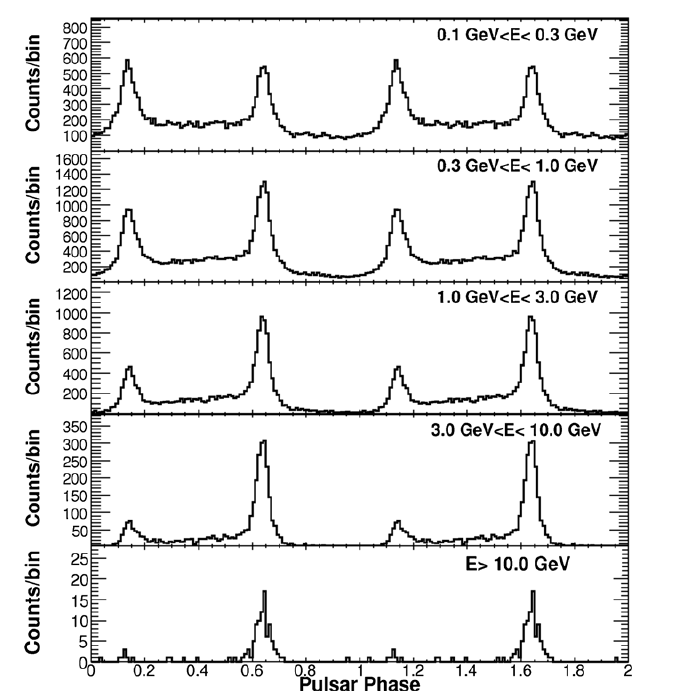
\includegraphics[width=0.7\textwidth]{pics/intro/geminga2.png}
  \caption[Gamma-ray lightcurves of Geminga]{Gamma-ray lightcurves of Geminga in
    five energy ranges, from {\it Fermi} observations
    \citep{abdo_fermi-lat_2010}. Two prominent peaks are seen in each rotation
    period.}
  \label{fig:geminga}
\end{figure}

Take the pulsar Geminga for example. It is the second brightest non-variable
$\mathrm{GeV}$ gamma-ray source in the sky. Its gamma-ray emission was first
discovered in the 1970s by the SAS-2 satellite
\citep{fichtel_high-energy_1975,kniffen_distribution_1975}. In contrast to the
Crab pulsar, Geminga is observed to be radio quiet, and is the first
representative of the class of radio quiet gamma-ray pulsars. As can be seen
from figure \ref{fig:geminga}, the gamma-ray peaks come in pairs in every
period, in contrast to the typical radio peaks in rotation powered pulsars,
suggesting that the gamma-ray emission comes from a very different region than
the radio emission.

After the launch of the {\it Fermi} satellite, the catalog of gamma-ray pulsars
exploded from 7 to well over 130 \citep{abdo_first_2010,abdo_second_2013}. The
gamma-ray pulsars are evenly divided into 3 groups: millisecond pulsars, young
radio-loud pulsars, and young radio-quiet pulsars. This discovery revolutionized
the way pulsars were studied. The pulsed gamma-ray emission typically carries
the highest fraction of the spin-down power $L_{d}$, therefore it can reveal the
most information about the particle acceleration and field structure in the
pulsar magnetosphere, much more so than the radio emission.

Many pulsars are also found to be X-ray sources, with pulsations detected in
many of them. The emission is usually made up of two components: a thermal
component from surface cooling or heated polar caps, and a non-thermal component
that is most likely magnetospheric due to synchrotron radiation
\citep{kaspi_isolated_2006}.


% The biggest difficulty in pulsar modeling is to account for this broadband
% radiation. A self-consistent model needs to explain not only the

\subsection{Theoretical models of the pulsar magnetosphere}
\label{sec:intro-pulsar-theory}

Despite the success of a simple vacuum dipole model, it proves to be extremely
difficult to obtain a more detailed self-consistent model of the pulsar
magnetosphere. The vacuum dipole model has a few problems. First, the
electric field from uni-polar induction effect gives a voltage that can
accelerate particles to $\sim 10^{14}\,\mathrm{V}$.
% TODO: how high voltage?
This voltage has two effects: it far exceeds the binding energy of electrons and
ions at the surface of the neutron star and can extract charged particles from
the stellar surface; it also accelerates the extracted particles to energies
that produce high-energy photons that are capable of interacting with the
intense magnetic field and convert into $e^{\pm}$ pairs, inducing a pair
cascade \citep{erber_high-energy_1966}.

As a result, it is not possible for the pulsar magnetosphere to be near vacuum.
A minimum corotating charge density is guaranteed around the pulsar which is
conventionally called the Goldreich-Julian density \citep{goldreich_pulsar_1969}:
\begin{equation}
  \label{eq:gj-density}
  \rho_\mathrm{GJ} = -\frac{\bOm\cdot \mathbf{B}}{2\pi c}\frac{1}{1 - (\Omega r/c)^2\sin^{2}\theta}
\end{equation}
where $\theta$ is the angle between magnetic axis and the rotation axis.
% TODO: expand on the GJ model

\subsubsection{Electrosphere}
\label{sec:electrosphere}

\begin{figure}[h]
  \centering
  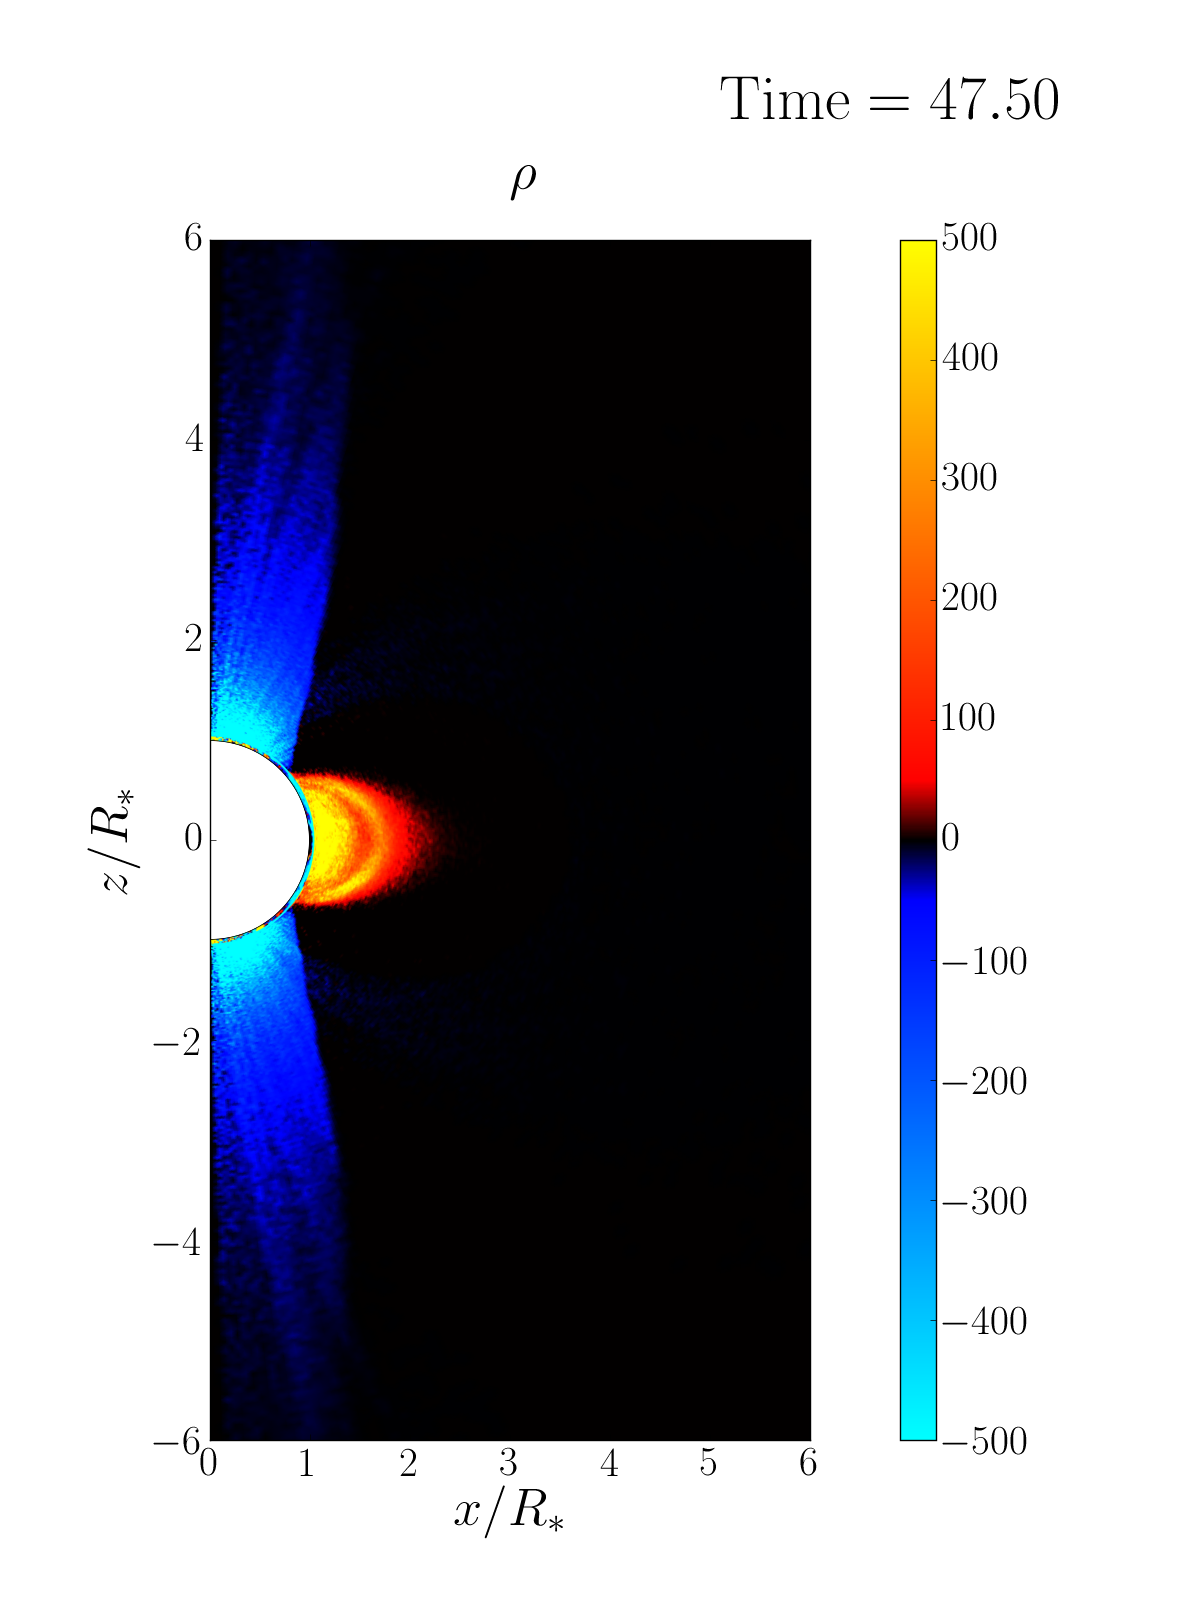
\includegraphics[width=0.54\textwidth]{pics/intro/electrosphere-new.png}
  \caption[Charge density distribution of the electrosphere of an aligned
  rotator.]{Charge density distribution of the electrosphere of an aligned
    rotator. Blue indicates negative charge and red indicates positive charge.
    Snapshot taken at time of $47.5R_{*}/c$ which is about 1.5 rotations of the
    star, and quasisteady state has been achieved.}
  \label{fig:electrosphere-intro}
\end{figure}

The problem of the Goldreich-Julian model is that charge lifted from the
surface alone is not sufficient to fill the magnetosphere with
$\rho_\mathrm{GJ}$. For an aligned rotator (magnetic axis aligned with rotation
axis), there exists an electrostatic equilibrium solution for the lifted charge
\citep{jackson_new_1976, krause-polstorff_pulsar_1985,
  krause-polstorff_electrosphere_1985}. The surface charge are lifted to form a
dome around both poles of the star, and a torus near the equator. In both the
dome and the torus $\mathbf{E}\cdot \mathbf{B} = 0$, whereas an unscreened
vacuum gap exists between them (figure \ref{fig:electrosphere-intro}). This
equilibrium solution has no outgoing Poynting flux, therefore no spin-down at
all. It is a dead pulsar.

It was speculated by \citet{spitkovsky_electrodynamics_2004} that oblique
rotators will be able to escape this fate due to diocotron instability
developing inside the torus, which leads to its slow expansion and eventually
reaching the light cylinder. This might jump-start the global current
circulation and allow the pulsar to start operating, but no simulation or
analytical results has been able to confirm this hypothesis. Furthermore,
\citet{petri_relativistic_2007} showed that this instability is suppressed by
relativistic effects that become important near the light cylinder.

Another problem with the electrosphere is that, a huge region with unscreened
parallel electric field exists between the dome and torus, capable of
accelerating stray particles to very high energies. These particles will be able
to produce curvature photons that are able to interact with the magnetic field
to produce $e^{\pm}$ pairs. Any cosmic ray particle can initiate this process
and produce a pair avalanche: the electrosphere solution is
unstable to pair creation.

Pair creation in the pulsar magnetosphere has been studied extensively since the
first theoretical models of the pulsar. There are several motivations for the
pulsars to produce abundant $e^{\pm}$ outflow. One stems from models attempting
to explain the radio emission which was central to pulsar studies for decades.
Most models for radio emission involve some plasma instability causing the
clumping of charges, which requires a dense quasi-neutral plasma, not the
charge-separated dome and torus in the electrosphere solution. Another
motivation is that the observed synchrotron radiation in the pulsar wind nebulae
calls for high amounts of $e^{\pm}$ pairs. In the case of Crab, the multiplicity
of pairs (number of $e^{\pm}$ pairs over the minimum Goldreich-Julian density)
is estimated to be $\mathcal{M} \gtrsim 10^{6}$ \citep{de_jager_gamma-ray_1996},
thus requiring the abundant pair creation in the magnetosphere.

Therefore, particle acceleration and pair creation has been a major topic in
theoretical pulsar research for decades. One of the challenges for any
theoretical model is that pair creation is naturally a self-limiting process:
the creation of abundant neutral plasma tends to screen the accelerating electric
field, thus reducing its efficiency or even turning off the process altogether.
Therefore it is difficult to have large regions in the magnetosphere where there
is unscreened parallel electric field: all pulsar particle acceleration models
involve a somewhat local ``gap'' where unscreened electric field keeps
accelerating particles, and pairs are created outside the ``gap'', unable to
screen it. It is not clear {\it a priori} whether the gap (or gaps) would be
static or periodically turning on and off, or whether the position would be
static in time.

\subsubsection{MHD and force-free models}
\label{sec:mhd-force-free}

Although the existence of gaps is crucial to fill the magnetosphere with the
required amount of plasma, it is instructive to study what happens to the
magnetosphere when plasma supply is not an issue. It makes sense to study the
approximation where plasma is so abundant as to screen all the parallel electric
field, $\mathbf{E}\cdot \mathbf{B}\approx 0$. The model assumes that the
inertial mass of the particles is much less than the magnetic field energy
$B^{2}/8\pi c$. This limit is called ``Force-free electrodynamics'' (FFE),
defined by the equation
\begin{equation}
  \label{eq:force-free}
  \rho \mathbf{E} + \frac{\mathbf{J}\times \mathbf{B}}{c} = 0
\end{equation}

The FFE condition is basically an equation for the current $\mathbf{J}$, which
closes the Maxwell equations. Force-free electrodynamics has no constraints on
the distribution of the plasma, other than the obvious requirement that $\rho =
\nabla\cdot \mathbf{E} / 4\pi$, and that $\mathbf{J}$ satisfies the force-free
equation \eqref{eq:force-free}. It assumes that enough plasma is always supplied
to maintain these two conditions as demanded by the electromagnetic field.

\begin{figure}[h]
  \centering
  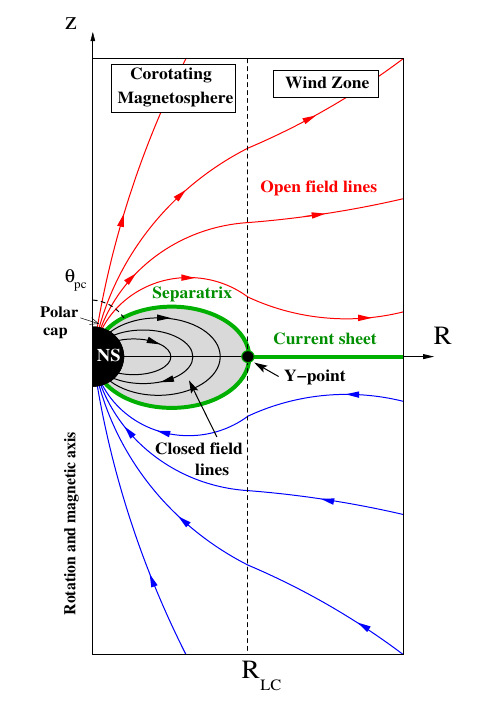
\includegraphics[width=0.5\textwidth]{pics/intro/force-free.png}
  \caption[The force-free magnetosphere.]{The force-free magnetosphere of an
    aligned rotator, from \citep{cerutti_electrodynamics_2016}. The
    magnetosphere is split into an open zone with outward Poynting flux and a
    closed zone with no energy flux. The separatrix between these zones forms a
    Y-shaped current sheet. }
  \label{fig:force-free}
\end{figure}

The force-free equation together with Maxwell equations form a closed system
and can be solved with the boundary condition of a rotating neutron star. The
equations were first solved numerically by \citet{contopoulos_axisymmetric_1999}
\citetext{see also e.g.\ \citealp{goodwin_idealized_2004};
  \citealp{gruzinov_power_2005}; \citealp{timokhin_force-free_2006};
  \citealp{parfrey_introducing_2012}}. The force-free solution of the pulsar
magnetosphere shows a few interesting features:
\begin{itemize}
\item An open zone where magnetic field lines extend to infinity, $B_{\phi}\neq
  0$ and current flows along the field lines. Poynting flux $\mathbf{S} =
  c\mathbf{E}\times \mathbf{B}/4\pi$ points outward along the poloidal $\mathbf{B}$
  field.
\item A closed zone where $B_{\phi} = 0$ and poloidal $j=0$, filled by plasma
  with density equal to $\rho_\mathrm{GJ}$. The closed zone corotates with the
  star, similar to the torus in the electrosphere solution. Poloidal magnetic
  field remains close to dipole configuration.
\item A thin Y-shaped current sheet that separates the close and open zones,
  with the Y-point close to the light cylinder.
\end{itemize}
These features are nicely summarized in figure \ref{fig:force-free}.

% TODO: Finish up the discussion for FFE, with 3D results and other stuff

However, FFE remains an approximation that glaringly breaks down in some regions
of the magnetosphere, namely inside the current sheets and in some inevitable
gaps where $\mathbf{E}\cdot \mathbf{B} \neq 0$ and particles are accelerated to
produce the plasma required by FFE. One can introduce finite resistivity and use
full resistive MHD approach to study the magnetosphere
\citep[e.g.][]{kalapotharakos_gamma-ray_2014}% TODO: ref
. However the issue of particle acceleration and formation of localized gaps
remain impossible to tackle in this framework.

\subsubsection{Gaps and pair cascade}
\label{sec:gap-models}

Several mechanisms of forming and maintaining localized gaps where particles are
accelerated have been proposed over the decades of pulsar research. The
classical picture was that the gap exists at the pulsar polar cap
\citep{sturrock_model_1971}. The motivation here is that, for open field lines
that penetrate the light cylinder, the plasma corotating on the field lines
can't move faster than the speed of light, therefore they have to lag behind the
corotating field lines at the light cylinder, bending the field lines backwards
to create a spiral-like pattern. This creates non-zero $\nabla\times \mathbf{B}$
therefore nonzero current along the open field lines: current flowing from the
polar cap region. \citet{sturrock_model_1971} considered space-charge limited
flow \citep{pierce_theory_1954} from the polar cap and estimated the voltage
drop from the surface of the star, and it was enough for particles to emit
energetic gamma-rays that can convert into $e^{\pm}$ pairs in the strong
magnetic field. The polar caps operate as ``guns'' shooting electron-positron
pairs along the open field lines and serve as the source of radio emission. From
the pulse profile, the width of the pulse is very small, indicating that radio
emission is coming from close to the star. Therefore the accelerating gap must
be close to the star as well.

\begin{figure}[h]
  \centering
  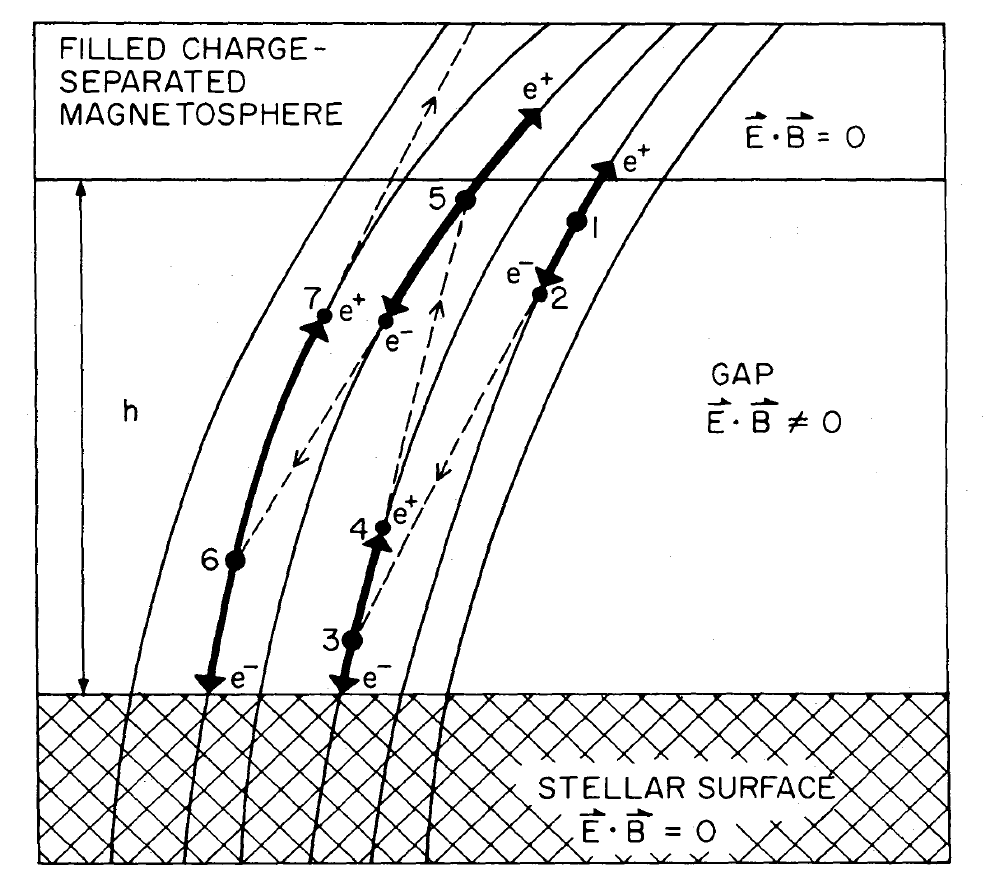
\includegraphics[width=0.55\textwidth]{pics/intro/ruderman-sutherland.png}
  \caption[Breakdown of the polar gap.]{Breakdown of the polar gap. The electric
    field accelerates positrons out of the gap and electrons towards the star
    \citep{ruderman_theory_1975}.}
  \label{fig:ruderman-gap-pic}
\end{figure}

Instead of space-charge limited flow, \citet{ruderman_theory_1975} considered
the case where positive charges need to be extracted from the star (e.g.\
anti-aligned rotator) but the electric field is not enough to overcome the
binding energy. In this case a vacuum gap near the polar cap is developed and a
pair discharge is initiated (figure \ref{fig:ruderman-gap-pic}). In the
originally vacuum gap, any stray electron or positron from say cosmic rays can
initiate this process of pair avalanche, where the stray particle is accelerated
and produces highly energetic curvature radiation. The photon propagates a short
distance before converting to an $e^{\pm}$ pair, which then serve as seeds for
the same process. The gap height $h$ is self-regulated such that this process
does not shut down, and keeps generating fresh plasma as they flow out to the
light cylinder to conduct the required current. The difference between these two
models lies in whether primary particles are extracted from the star, or
recycled from the previous generation of created pairs (figure
\ref{fig:polar-gaps}).

Another gap model is the outer gap, proposed by \citet{cheng_energetic_1986},
which originate from the region in the magnetosphere where $\rho_\mathrm{GJ} =
0$, or in other words, $\bOm\cdot \mathbf{B} = 0$. A charge-separated flow from
the star cannot penetrate this boundary since the space charge density changes
sign here. Therefore, if the current from the star is carried by particles
extracted from the surface, this is where an unscreened gap will develop,
leading to a pair discharge in the outer magnetosphere.

\begin{figure}[h]
  \centering
  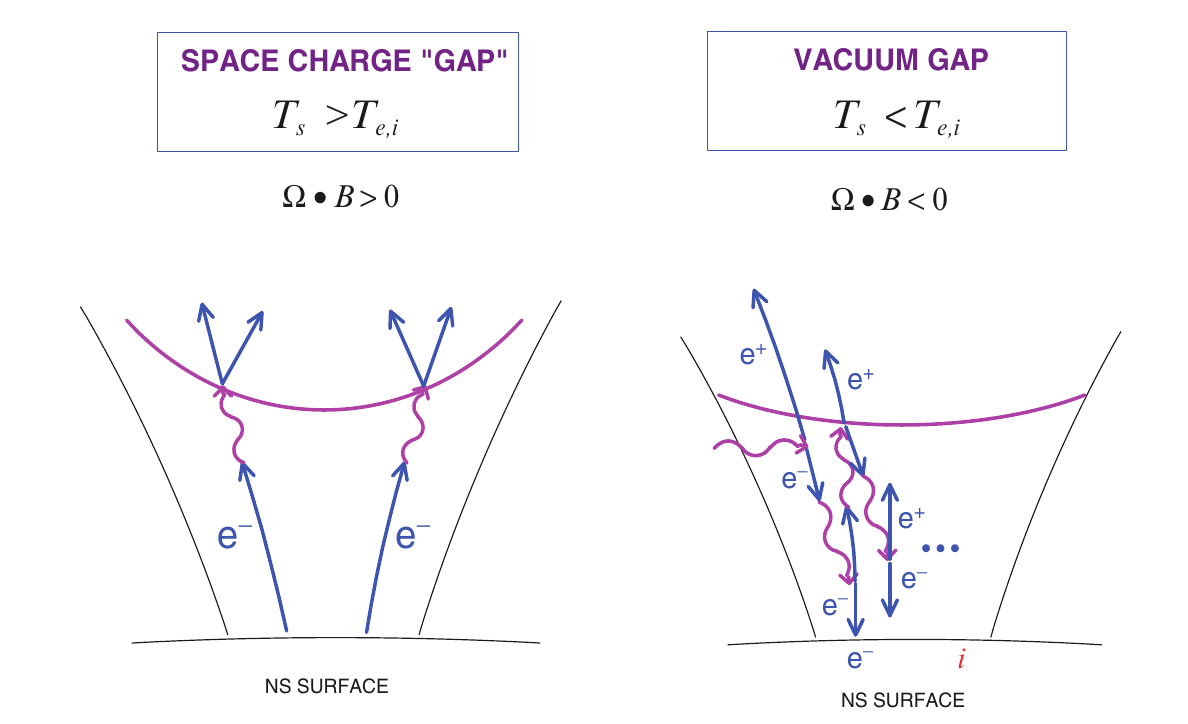
\includegraphics[width=0.7\textwidth]{pics/intro/polar-gaps.png}
  \caption[Space-charge limited polar gap and vacuum polar gap.]{Space-charge
    limited polar gap vs vacuum polar gap \citep{harding_high-energy_2009}.}
  \label{fig:polar-gaps}
\end{figure}

This outer gap model predicts a double pulse gamma-ray light curve that is
similar to that observed in Crab and Vela, which is one of the reasons that it
is popular among observers in explaining the emission from gamma-ray pulsars.
However, the outer gap picture assumes a vacuum dipole field configuration even
up to the outer magnetosphere, whereas we know from FFE simulations that the
field structure is significantly altered by the presence of plasma.
\citet{bai_modeling_2010} used the more realistic field configuration from 3D
FFE calculations and showed that in fact this traditional outer gap model is
capable of producing only one peak under general conditions because a large
fraction of open field lines do not cross the null surface.

\begin{figure}[h]
  \centering
  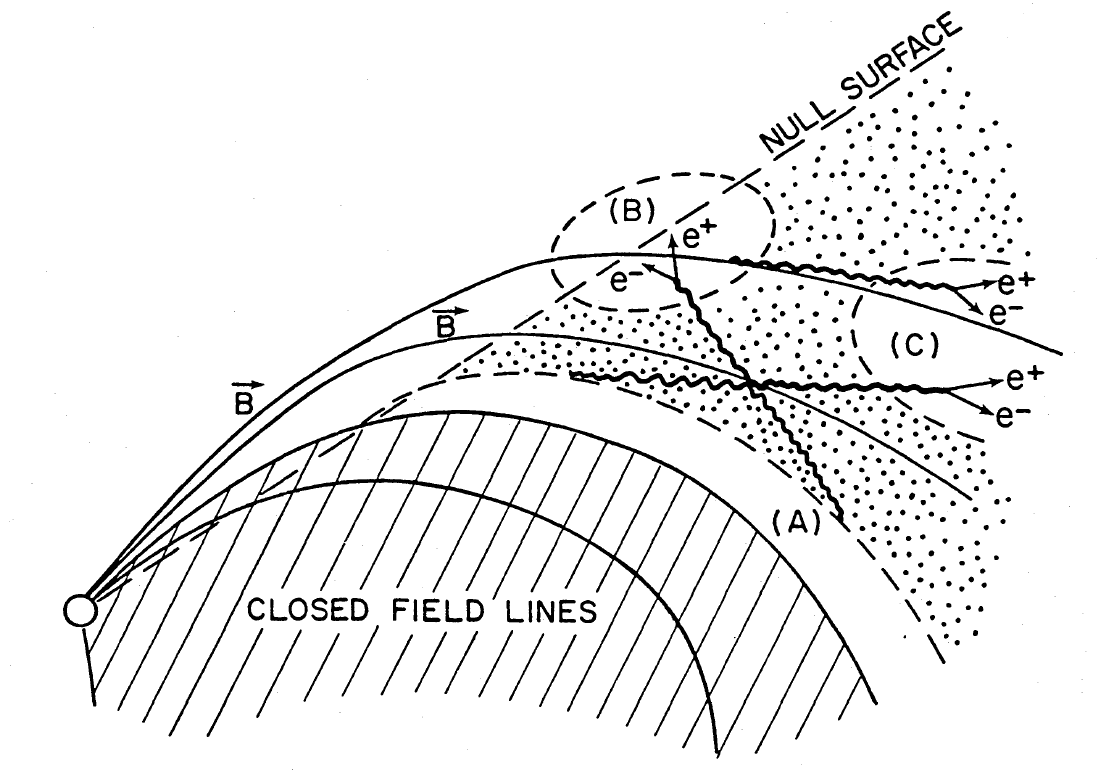
\includegraphics[width=0.55\textwidth]{pics/intro/outer-gap.png}
  \caption[Outer gap]{Outer gap, from \citet{cheng_energetic_1986}.}
  \label{fig:outer-gap}
\end{figure}

Another gap model is the slot gap which is an extension of the polar gap along
the last closed field line (figure \ref{fig:slot-gap}). It also aims at
explaining the high energy gamma-ray emission from pulsars. The original idea
was proposed by \citet{arons_pair_1979} who realized that the acceleration
potential varies significantly across the polar cap, resulting in an extended
pair creation front almost parallel to the last closed field line. This gap is
capable of slowly accelerating particles along the field lines to high energies
at a much higher altitude than the polar cap gap, producing gamma-ray emission
from curvature radiation.

Despite the decades of effort, a global picture of the pulsar magnetosphere with
both a realistic FFE field structure and a gap that self-consistently generate
the required plasma is still lacking. The physics of the pulsar magnetosphere
is surprisingly rich and it is important to take into account the interplay
between plasma physics and radiative transfer at very high energies. A global
simulation from first principles is needed to fully understand how pulsars work.

\begin{figure}[h]
  \centering
  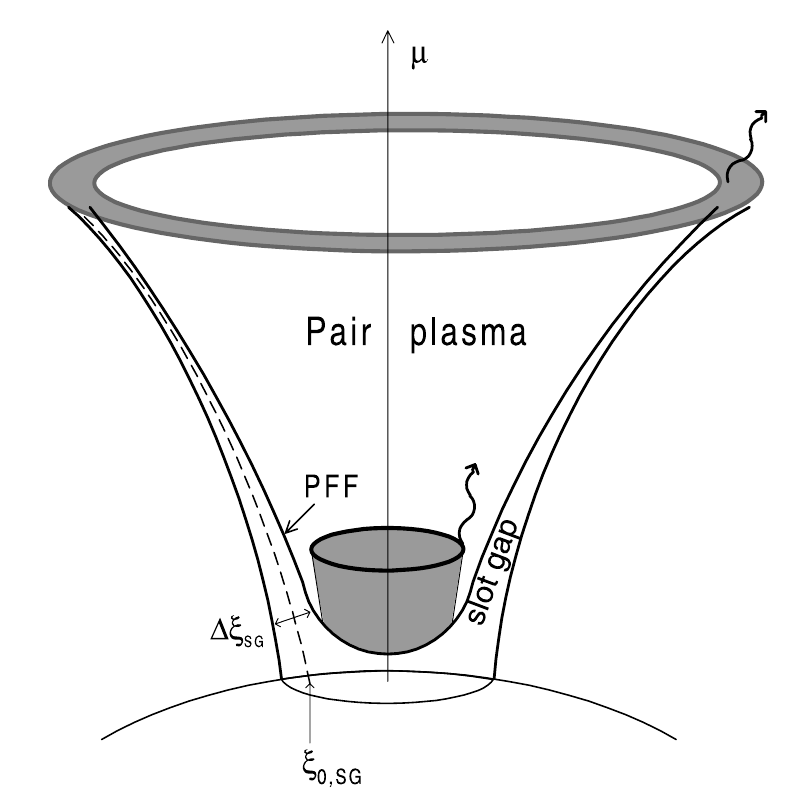
\includegraphics[width=0.5\textwidth]{pics/intro/slot-gap2.png}
  \caption[Slot gap geometry.]{Slot gap geometry \citep{muslimov_extended_2003}.
  The gap exists between the plasma created in the polar cap cascade and the
  closed field line zone which is filled with plasma extracted from the star.}
  \label{fig:slot-gap}
\end{figure}

\section{Magnetars}
\label{sec:intro-magnetars}

% TODO: Introduce magnetars, and open up the historical observation discussions
Magnetars are a class of neutron stars with very drastic variability in X-ray
and soft $\gamma$-ray bands. They exhibit recurrent bursts, flares, and
sometimes giant bursts that can briefly outshine entire galaxies in the X-ray
luminosity. Their activity is powered by the decay of their strong magnetic
field, which is typically 100 times higher than ordinary rotation-powered
pulsars.

\subsection{Early Observations}
\label{sec:intro-magnetar-observation}

Historically ``magnetar'' was not the name given upon its discovery. The first
reports for magnetar activity can be traced back to 1979. The Venera 11 and
Venera 12 space probes recorded 3 repeated soft gamma-ray bursts from a single
source B1900+14 \citep{mazets_soft_1979}. It was initially believed to share
similar origins with other short gamma-ray bursts. During the same year, the
space probes also recorded hard X-ray bursts from a different source FXP 0520-66
in Dorado, which was apparently an X-ray pulsar from the beginning
\citep{mazets_observations_1979}. These sources were designated ``Soft Gamma-ray
Repeaters'' (SGRs).

Several years later another SGR 1806-20 was found in our galaxy, and it
underwent repeated bursts on the order of 100 times over less than 10 years
\citep{kouveliotou_smm_1987,laros_new_1987}. It was also the first SGR that had
a measured spin-down rate \citep{kouveliotou_x-ray_1998}. The dipolar magnetic
field computed by the simple spin-down formula \eqref{eq:surface-B-field} gives
a surface field strength of $8\times 10^{14}\,\mathrm{G}$, much higher than
typical rotation-powered pulsars discovered yet. The ultrastrong magnetic field
of SGR 1806-20 was in line of the magnetar model proposed by
\citet{duncan_formation_1992}. In their paper they coined the term ``magnetar''
to describe young neutron stars with high magnetic field ($10^{14}\sim
10^{15}\,\mathrm{G}$), and argued that magnetars are the sources of SGRs, where
the bursts are powered by spontaneous decay of the strong magnetic field of the
magnetar. Being young objects with age $10^{3}\sim 10^{4}$ years, magnetars are
still dynamically evolving internally and building up stress that can lead to
breaking of the crust, releasing a significant amount of energy into the
magnetosphere in the form of Alfvén waves, which then powers the X-ray and soft
gamma-ray emission.

Another class of magnetars was discovered separately and recognized as
``Anomalous X-ray Pulsars'' (AXPs). In 1980 it was reported that in the
region CTB 109 there was ``an extraordinary new celestial X-ray
source'' which was a supernova remnant \citep{gregory_extraordinary_1980}. Soon
it was found that this source displays very strong pulsation with a period of
$\sim 3.5\,\mathrm{s}$ \citep{fahlman_x-ray_1981}. More X-ray pulsars were
subsequently discovered that also have similar few-second period, and share
similar soft X-ray spectra.

Thompson and Duncan speculated that AXPs may be related to SGRs, and predicted
that long-term observations of AXPs might lead to bursting behavior
\citet{thompson_soft_1996}. This was then confirmed by
observation. %TODO: flesh out this paragraph
Now both AXPs and SGRs are recognized under the same umbrella known as
magnetars. Among the $\sim 30$ known magnetars, a more intrinsic
characterization is their quiescent luminosity. {\it Transient magnetars} are
typically only detected during their bursts, while {\it persistent magnetars}
are bright even in their quiescent state. They are usually what used to be
associated with AXPs, showing strong and persistent pulsed X-ray emission.

\subsection{Observational Puzzles}
\label{sec:magnetar-puzzles}

\begin{figure}[h]
  \centering
  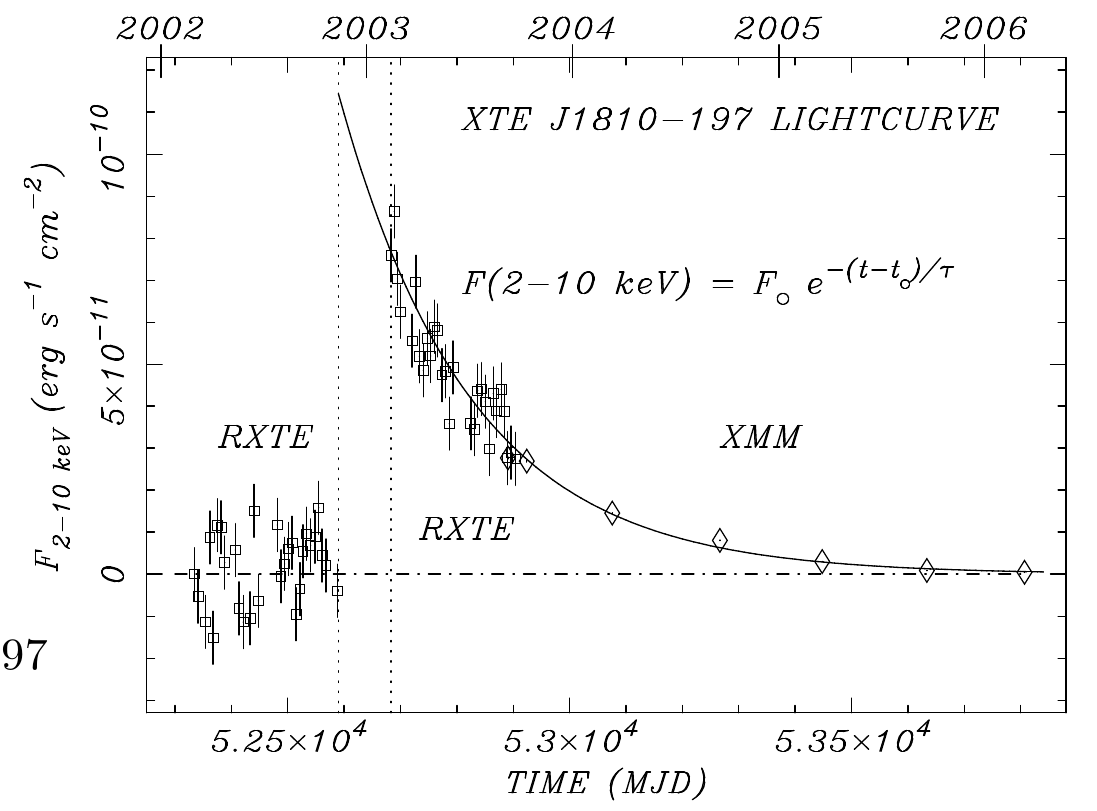
\includegraphics[width=0.7\textwidth]{pics/intro/transient.png}
  \caption[Light curve for the outburst from transient magnetar XTE J1810-197]{Light curve for the outburst from transient magnetar XTE J1810-197 \citep{gotthelf_anatomy_2007}.}
  \label{fig:outburst-light-curve}
\end{figure}

For transient magnetars, apart from short and irregular bursts that are the
signature of SGR activity, they also show large outbursts with short rise time
and long decay. A classic example is the transient magnetar XTE J1810-197, which
underwent an outburst in early 2013 \citep{ibrahim_discovery_2004}, and its
luminosity slowly decayed to quiescent levels over several years (figure
\ref{fig:outburst-light-curve}). \citet{gotthelf_anatomy_2007} found that the
X-ray spectrum of the magnetar during outburst can be fitted by 2 blackbody
components, one with lower temperature and larger area, which subsequently cooled
but expanded to cover almost the entire star, and another with smaller area and
higher temperature, {\it shrinking} over time (figure
\ref{fig:shrinking-hotspot}). This has very important implications for modeling
the magnetar outburst: the model should be able to explain the origin of the
hotspot, as well as the reason and timescale of its shrinking.

\begin{figure}[h]
  \centering
  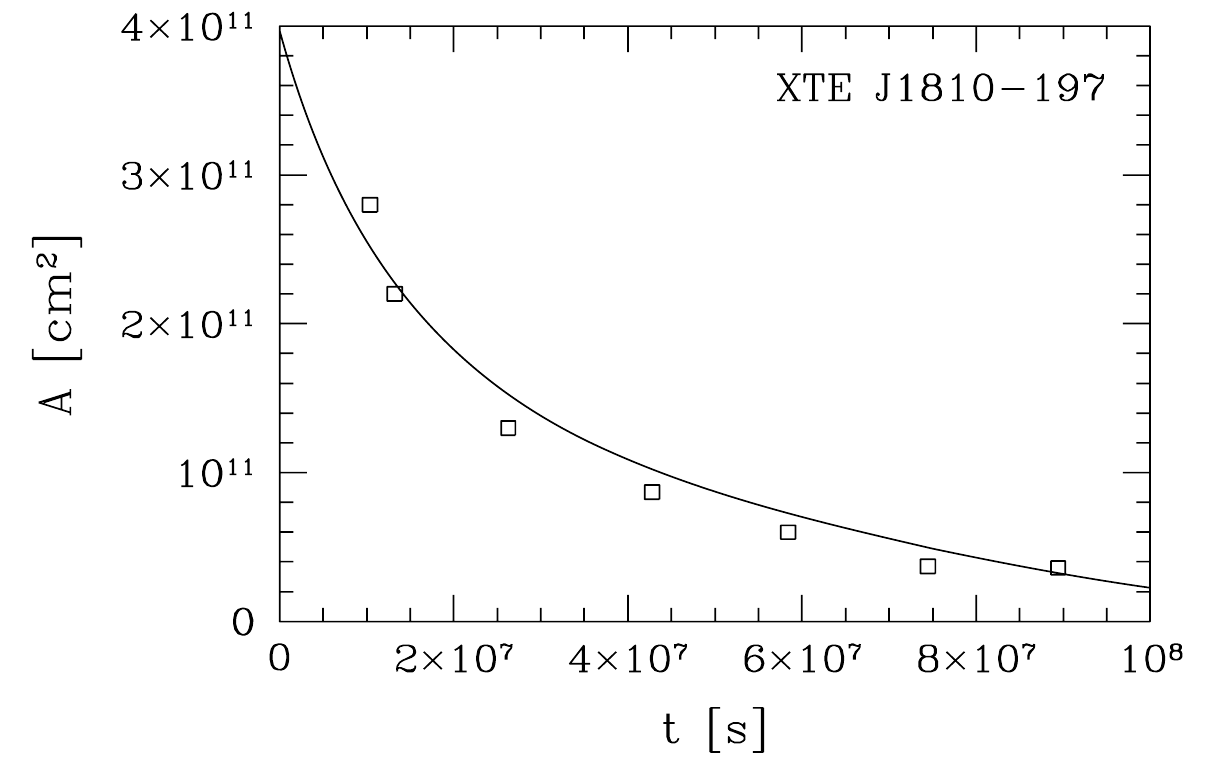
\includegraphics[width=0.7\textwidth]{pics/intro/shrink-spot.png}
  \caption[Evolution of the fitted area of the hot component in the X-ray
    spectrum of XTE J1810-197.]{Evolution of the fitted area of the hot component in the X-ray
    spectrum of XTE J1810-197. The area shrunk by a factor of more than 8 over
    the course of a few years.}
  \label{fig:shrinking-hotspot}
\end{figure}

The shrinking hotspot feature was not only seen in one transient magnetar.
Figure \ref{fig:hotspots} shows the evolution of luminosity versus the area of
the fitted hotspot for 7 of the known transient magnetars for which a hotspot
has been identified. All seem to follow a similar trajectory over the $A$-$L$ plane.

\begin{figure}[h]
  \centering
  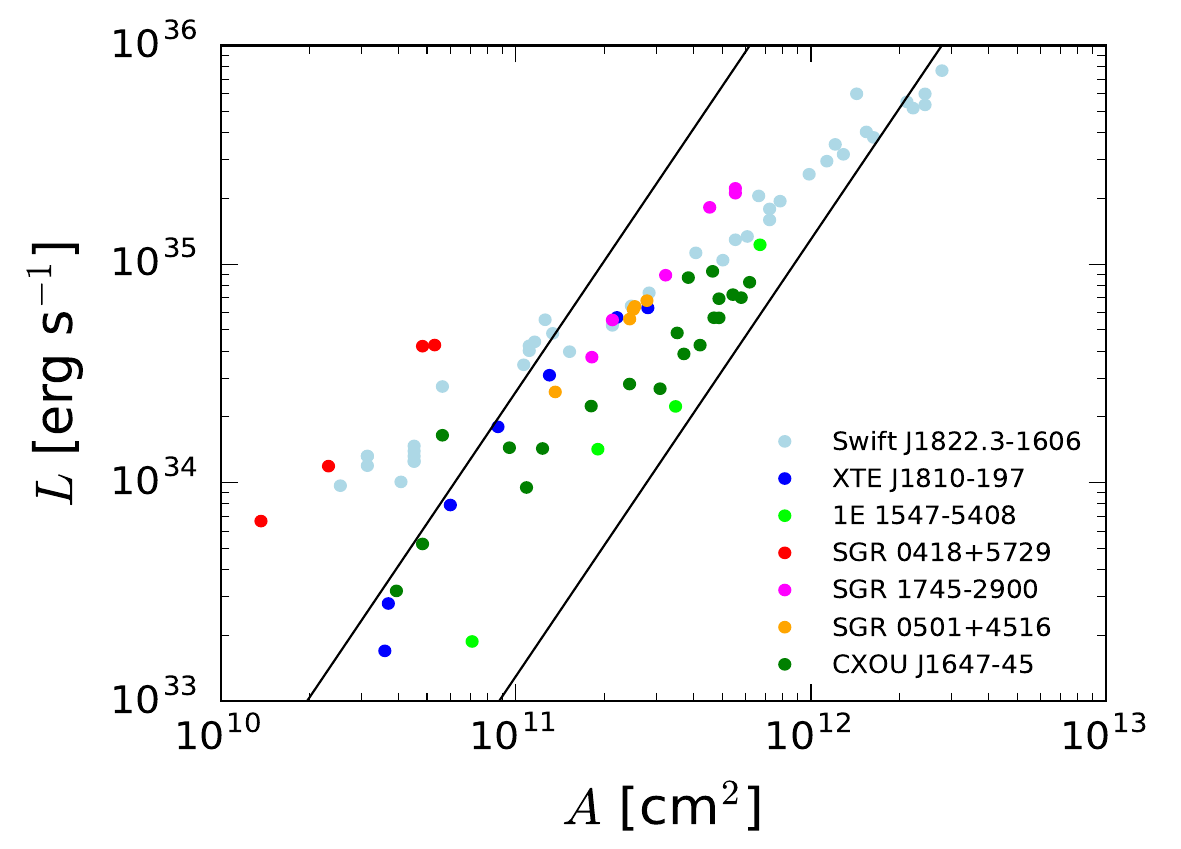
\includegraphics[width=0.7\textwidth]{pics/intro/hot-spot.png}
  \caption[The evolution of hotspots observed on transient magnetars following
    outbursts.]{The evolution of hotspots observed on transient magnetars following
    outbursts. The hotspots shrink and become dimmer over time, tracking a
    similar trajectory on the $A$-$L$ plane. \citep{beloborodov_magnetar_2016}}
  \label{fig:hotspots}
\end{figure}

Persistent magnetars also pose an important observational puzzle. Previously
AXPs were observed to have a soft X-ray spectrum that can be described by a
blackbody plus power law. The X-ray spectrum turns down and was predicted to be
not detectable above $10\,\mathrm{keV}$. However \citet{kuiper_discovery_2006}
discovered hard spectral tails for 3 persistent magnetars 1RXS J1708$-$4009, 4U
0142+4009, and 1E 2259+586. This turned out to be a great surprise. Furthermore
the X-ray component above $10\,\mathrm{keV}$ is extraordinarily hard and extends
up to and beyond $150\,\mathrm{keV}$. Later \citet{enoto_broadband_2010}
reported the identification of the hard X-ray tail in 7 magnetars including 2
transient magnetars in outburst states, namely SGR 0501+4516
\citep{enoto_wide-band_2010} and 1E 1547.0$-$5408 \citep{enoto_suzaku_2010}. By
now it has been recognized that this soft emission plus hard tail is a common
feature for magnetars. This high-energy nonthermal component dominates the
emission energy, and is thought to be of magnetospheric origin. This hard X-ray
component is another interesting puzzle posed by the magnetar observations.

\begin{figure}[h]
  \centering
  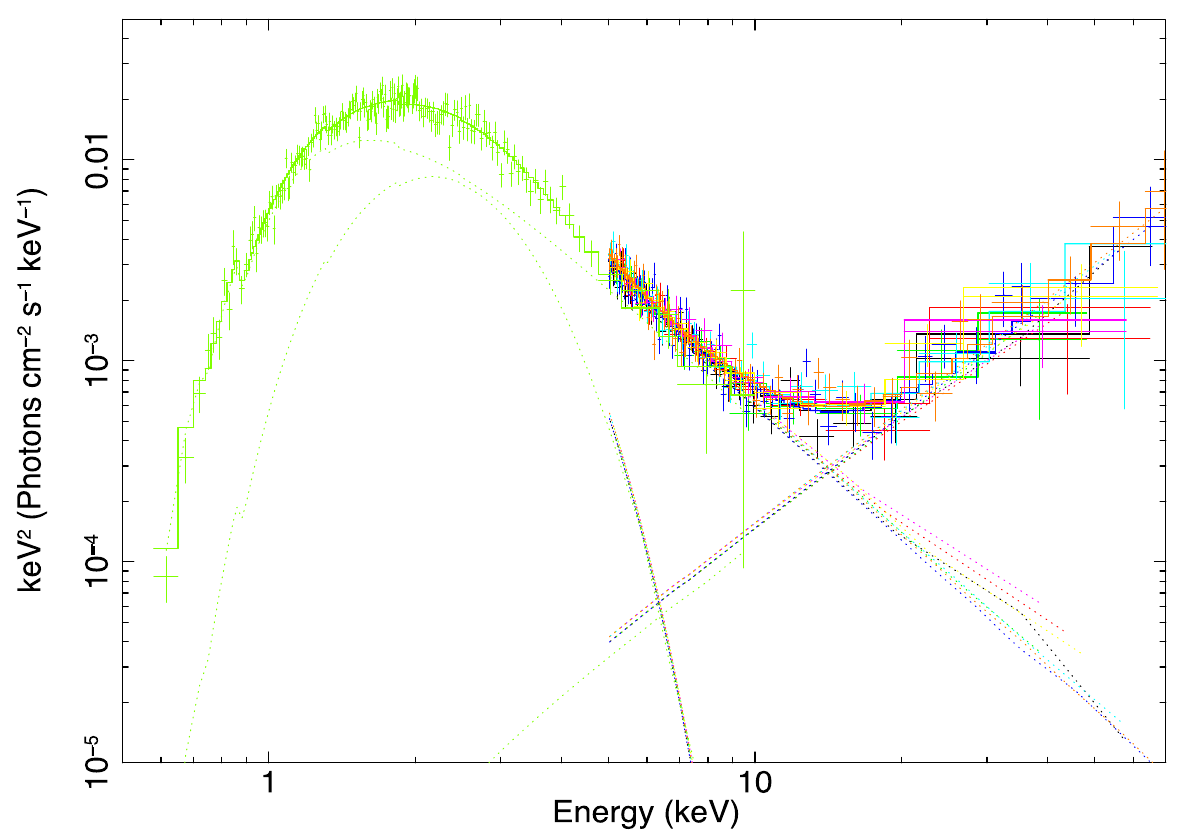
\includegraphics[width=0.6\textwidth]{pics/intro/hard-x-ray.png}
  \caption[X-ray spectrum of 1E 2259+586.]{X-ray spectrum of 1E 2259+586
    \citep{vogel_nustar_2014}. The graph truncates at 100keV but the spectrum
    extends above that.}
  \label{fig:magnetar-hard-x-ray}
\end{figure}


\subsection{Theoretical Models}
\label{sec:intro-magnetar-theory}

% Here describe the crustal shear and magnetospheric twist model. Describe the
% particle flow, acceleration. Double layer. Resonant scattering. Go into more
% detail in the appendix.
Magnetars are all very young neutron stars that have very high surface magnetic
field. The interior of a neutron star is an excellent conductor, and magnetic
field is practically frozen into the material. Field evolution is a result of
the evolution of electron fluid coupled to the ion and neutron fluids, which can
be described by two processes: ambipolar diffusion and Hall drift
\citep{goldreich_magnetic_1992}. These processes move magnetic field lines and
can build up magnetic stress inside a neutron star, which could lead to a sudden
failure of the crust and ejection of this energy into the magnetosphere
\citep{thompson_soft_1995, thompson_giant_2001}. An alternative way of
triggering this release is a slow build up of the stress due to a gradual
deformation of the magnetosphere, as long as this process is faster than the
rate it is damped \citep{lyutikov_magnetar_2006}.

In any case, the result of surface shear is the deformation of the external
magnetosphere from the quasisteady configuration, twisting the magnetic field
lines and launching Alfven waves into the magnetosphere, creating regions where
$\nabla\times \mathbf{B} \neq 0$. Current will flow along the twisted field line
bundle, $\mathbf{j} = (c/4\pi)\nabla\times \mathbf{B}$. A strongly twisted
magnetosphere is prone to global instability \citep{uzdensky_shear-driven_2002},
and will result in the formation of an equatorial current sheet, where magnetic
reconnection happens and energy is released violently in a short time scale.
This was seen in force-free simulations carried out by
\citep{parfrey_dynamics_2013}.

\begin{figure}[h]
  \centering
  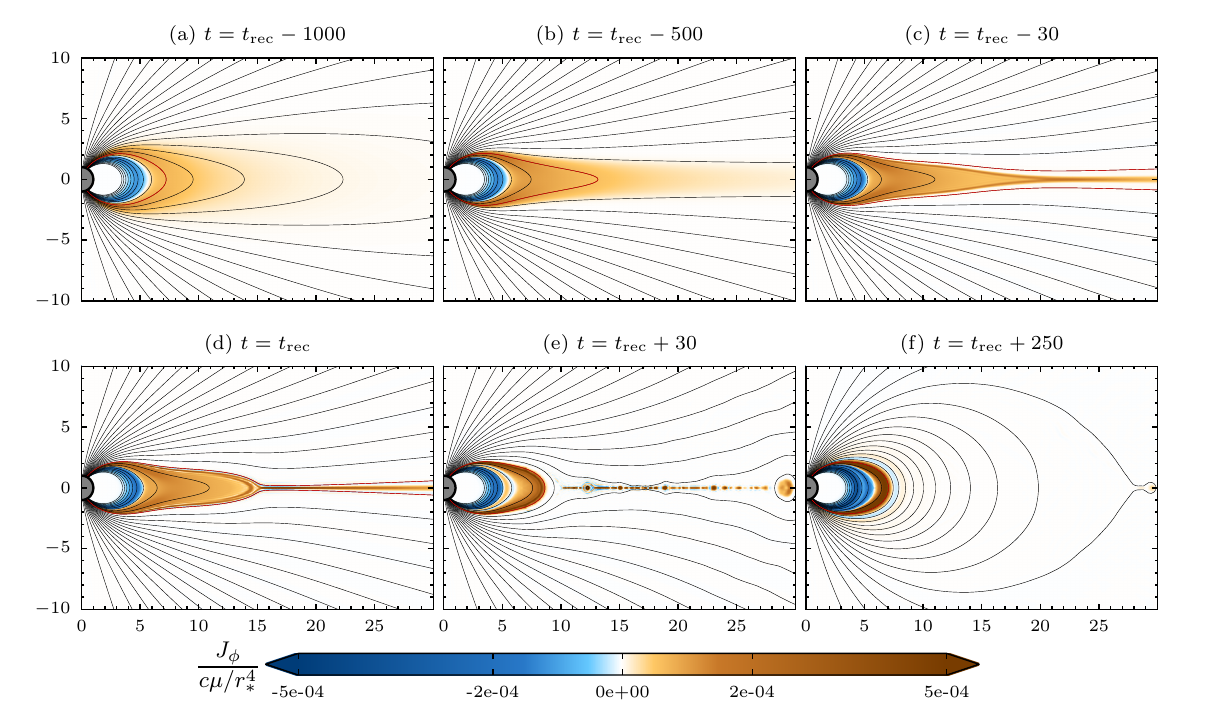
\includegraphics[width=0.8\textwidth]{pics/intro/ffe-giant-flare.png}
  \caption[Formation of the equatorial current sheet in over twisted magnetar
    magnetosphere.]{Formation of the equatorial current sheet in over twisted magnetar
    magnetosphere. Color shows toroidal current density. Time is indicated in
    units of light crossing time of the star. From \citep{parfrey_dynamics_2013}}
  \label{fig:overtwisted-magnetar}
\end{figure}

When the twist is not as dramatic, the current bundle can be long-lived. This
should feed the observed long decay of the X-ray luminosity after an outburst
event. \citet{beloborodov_corona_2007} studied the dynamics of the current loop,
concluding that electric field will be induced to extract particles from the
surface of the star, accelerate them, and initiate a pair avalanche similar to
that in pulsar magnetosphere. The current loop acts as a ``corona'' of the
magnetar. Particles are lost to the stellar surface over one light crossing time
of the system and are constantly replenished from pair creation. The main
channel for pair creation is from photons upscattered resonantly: electrons
moving at Lorentz factor of $\sim 1000$ will see a background sea of soft X-ray
photons of a few keV, which when boosted into the rest frame of the electron
matches the energy to excite the particle from the ground Landau level to the
first excited level. When this resonance condition is satisfied, the electron
will be able to absorb the photon and re-emit it. The re-emitted photon will see
an energy boost of $\sim \gamma^{2}$ in the lab frame, and capable of creating
$e^{\pm}$ pairs by means of magnetic conversion.

The lifetime of the magnetar twist is determined by the acceleration voltage
induced in the $j$-bundle, which is in turn governed by the threshold of pair
discharge. However the self-regulation of this process is a non-trivial problem.
It was also discovered by \citet{beloborodov_untwisting_2009} that the process
of untwisting proceeds in an interesting manner. A current cavity develops first
in the inner magnetosphere, which subsequently expands and erasing the current
carrying part of the twisted field lines. This effectively means that the
cross-sectional area of the current bundle shrinks as the magnetosphere untwists
over time. If the hotspot seen in the blackbody spectrum after an outburst is to
be mapped to the footprint of the $j$-bundle, then this provides a natural
explanation of the shrinking hotspot.

Resonant scattering not only provides a means to generate high-energy photons
that can convert to pairs, it also affects the relativistic flow of the pair
plasma along the twisted field lines. \citet{beloborodov_mechanism_2013}
proposed a mechanism for the hard X-ray component seen in the magnetar spectrum.
Particles are extracted from the star and undergo acceleration to $\gamma\gg
10$. In this region the resonantly scattered photons interact with the local $B$
field and quickly convert to $e^{\pm}$ pairs, effectively pair loading the
plasma with multiplicity $\mathcal{M}\sim 100$. When the flow gets to a region
with weaker magnetic field, the resonantly scattered photon will be able to
escape to form the observed X-ray spectrum (figure \ref{fig:magnetar-loop}).
Finally at the tip of the magnetic loop near the equator, the radiative drag
will be strong enough to stop the particles to $\gamma \sim 1$. The particles
suspended near the equator will serve as a reflector for the X-ray photons from
the star. They might also be able to generate radio emission which is seen in
some of the magnetars.

\begin{figure}[h]
  \centering
  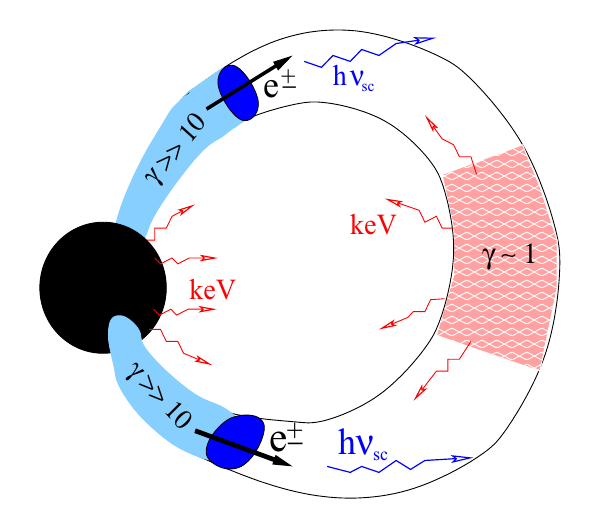
\includegraphics[width=0.5\textwidth]{pics/intro/magnetar-loop.png}
  \caption[Sketch of a twist magnetic loop.]{Sketch of a twist magnetic loop.
    Particles are accelerated in the blue region and resonantly scatter photons
    reflected from the pink region. The upscattered photons convert to pairs
    near the star, but can escape in the white region to form the observed X-ray
    spectrum \citep{beloborodov_mechanism_2013}.}
  \label{fig:magnetar-loop}
\end{figure}

The picture described above was successfully used to fit the phase-resolved
spectra of several magnetars \citep{hascoet_phase-resolved_2014}. The narrowness
of the fitted parameters space is a strong indication for the correctness of the
model. It would be a decisive confirmation if the model can be reproduced in a
first-principle kinetic simulation.

\section{This Dissertation}
\label{sec:intro-outline}

In this dissertation we will attempt to study the problem of particle
acceleration and global structure of the magnetosphere of pulsars and
magnetars using numerical experiments. Most of the work is done using a computer
code named {\it Aperture} that I developed in the course of the PhD.

Chapter \ref{chap:pic} will be devoted to a detailed exposition of the
particle-in-cell method, which will be the basic numerical tool for our study.
We will introduce the {\it Aperture} code, and explain its novel features, as
well as providing some tests to demonstrate its correctness.

Chapter \ref{chap:polar-cap} will focus on a local study of the pulsar
polar cap. We will look at the region well within the pulsar magnetosphere, and
approximate the geometry as 1D. We will discuss implications of this
approximation, and what we can and can not learn from this local study.

Chapter \ref{chap:pulsar} will study the global pulsar magnetosphere, motivated
by the study of the polar cap particle acceleration. We will discuss the
result from global PIC simulations and contrast it with force-free results, and
study the condition under which a pulsar can sustain itself through pair discharge.

Chapter \ref{chap:magnetar} will study the twisted magnetosphere of magnetars
and attempt to answer how particles are accelerated in the current bundle and
what regulates the overall voltage.

Chapter \ref{chap:explorations} will contain some exploratory extensions of the
PIC code into the general relativistic regime.

% Local Variables:
% TeX-master: "../thesis"
% zotero-collection: #("16" 0 2 (name "Thesis"))
% End:
